% --- DVA218 lab 3 -------------------------
% | Information:                           |
% | If you only want to write the text and |
% | don't want to change settings place    |
% | go to the row that have the comment    |
% | -- Start writing here---               |
% ------------------------------------------

% ------------- START SETTINGS -------------------------------
\documentclass[conference]{IEEEtran}
\usepackage{blindtext, graphicx}

\ifCLASSINFOpdf
\else
\fi

% A couple of useful packages
\usepackage[table]{xcolor}
\usepackage{listings}
\usepackage{color}
\usepackage{amsmath}
\usepackage{subfiles}
 
 % Programming color don't touch without permissions.
\definecolor{codegreen}{rgb}{0,0.6,0}
\definecolor{codeblue}{HTML}{0073e6}
\definecolor{codegray}{rgb}{0.5,0.5,0.5}
\definecolor{commentgray}{rgb}{0.6,0.6,0.6}
\definecolor{codepurple}{rgb}{0.58,0,0.82}
\definecolor{stringblue}{HTML}{0073e6}
\definecolor{stringpurple}{HTML}{ff99ff}
\definecolor{backcolour}{rgb}{1,1,1}
 
\lstdefinestyle{mystyle}{
    backgroundcolor=\color{backcolour},   
    commentstyle=\color{commentgray},
    keywordstyle=\color{codeblue},
    numberstyle=\tiny\color{codegray},
    stringstyle=\color{codegreen},
    basicstyle=\footnotesize,
    breakatwhitespace=false,         
    breaklines=true,                 
    captionpos=b,                    
    keepspaces=true,                 
    numbers=left,                    
    numbersep=5pt,                  
    showspaces=false,                
    showstringspaces=false,
    showtabs=false,                  
    tabsize=2
}
 
\lstset{style=mystyle}
\lstset{language=c} % C is the default language in listings.

\usepackage{mdwmath}
% --- packages for state machine ----
\usepackage{tikz}
\usetikzlibrary{arrows,automata}
% --- end state -------------------------

\begin{document}
\title{DVA218 - Assignment 3a}
\author{\IEEEauthorblockN{Hampus Baaz}
\and
\IEEEauthorblockN{Wicktor L{\"o}w}
\and
\IEEEauthorblockN{Magnus S{\"o}rensen}}
% make the title area
\maketitle

${}$\hspace{5em}

%\IEEEpeerreviewmaketitle

%\vspace{10 mm}

% --- END SETTINGS --------------------------------------------

%  |~~~Start writing here----------------
%  |--->
\section{Introduction}
This is the first part of two in an assignment with the goal to create a reliable and efficient transport protocol on top of UDP. This first part contains state-machines for the different modules we will be implementing later in the code. There are three different modules, a connection with a three-way handshake, a sliding window protocol with selective acknowledgements and a teardown protocol. Each module will be described with two state machines, one for the sender (client) and one for the receiver (server).

\section{State machines}
Below we have six different Moore-styled state machines with figures and text describing how our modules we will implement, work.

\subsection{Three-way handshake - Client}
  
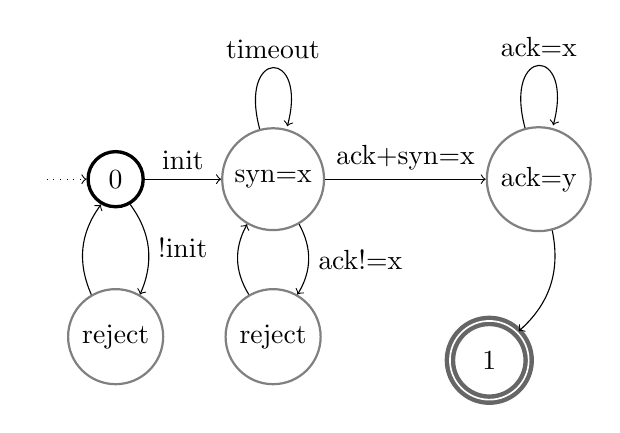
\begin{tikzpicture}
[
init/.style={circle, draw=black!100, very thick, minimum size=7mm,node distance=2cm},
state_split/.style={circle, draw=gray!100, thick, minimum size=7mm,node distance=2cm},
state/.style={circle, draw=gray!100, thick, minimum size=7mm,node distance=2cm},
final/.style={circle, double, draw=black!60,  ultra thick, minimum size=10mm,node distance=23mm}
]
%Nodes
\node[init]             (start)                         {0};
\node                   (em)        [left of=start]     {};
\node[state_split]      (reject)    [below of=start]    {reject};
\node[state_split]      (synx)      [right of=start]    {syn=x\nodepart{lower} 2};
\node[state]      (end)       [right of=synx, right=7mm]     {ack=y};
\node[state_split]      (rejected)  [below of=synx]     {reject\nodepart{lower}3};
\node[final]            (end2)      [below of=end, left=1mm]      {1};


%Lines
\draw[dotted, ->] (em.east) -- (start.west);
\path[->] 
(start)   edge [bend left]        node[right]     {!init}     (reject)
(reject)  edge [bend left]        node[left]      {}         (start)
(start)   edge                    node[above]     {init}      (synx)
(synx)    edge [bend left]        node[right]     {ack!=x}      (rejected)
(rejected) edge [bend left]       node[left]      {}        (synx)
(synx)    edge                    node[above]     {ack+syn=x}     (end)
(end)     edge [loop above]       node            {ack=x}     (end)
(synx)  edge    [loop above]      node            {timeout}    (synx)
(end)   edge    [bend left]       node            {}         (end2);
\end{tikzpicture}

\\
The client start out by sending a synchronisation package (sync) to the server, this package contains information for the sliding window protocol, e.g. window size and number of packages it wants to send. After sending this sync it will wait to receive an acknowledgement (ACK) from the server. If it receives a wrong ACK it will proceed to send a reject back to the server then send a new sync package, if it takes to long time and goes to timeout it will also resend the sync. When it finally receives the right ACK it will establish a connection to the server. In the final stage, the client will discard any ACK:s that might have fallen behind and come in late.  
\subsection{Three-way handshake - Server}
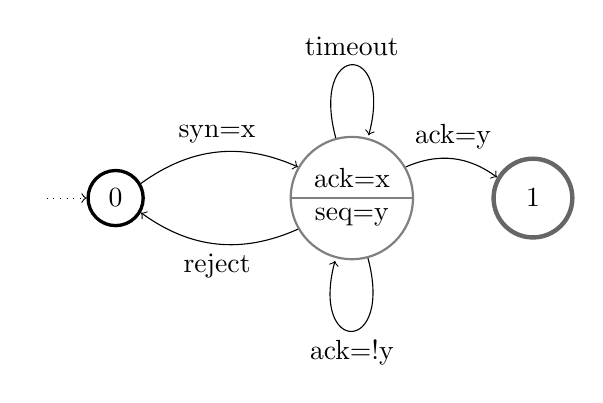
\begin{tikzpicture}
[
init/.style={circle, draw=black!100, very thick, minimum size=7mm,node distance=2cm},
state_split/.style={circle split, draw=gray!100, thick, minimum size=7mm,node distance=3cm},
state/.style={circle, draw=gray!100, thick, minimum size=7mm,node distance=2cm},
final/.style={circle, draw=black!60,  ultra thick, minimum size=10mm,node distance=23mm}
]
%Nodes
\node[init]     (start)                         {0};
\node           (init)        [left of=start]     {};
\node[state_split]    (synx)      [right of=start]    {ack=x\nodepart{lower}seq=y};
\node[final]    (end)       [right of=synx]     {1};



%Lines
%\draw[->] (start.east) -- (synx.west);
%\draw[->] (synx.east) -- (end.west);
%\path[->] (start)  edge [loop above] node {a} (start); 
\draw[dotted, ->] (init.east) -- (start.west);
\path[->] 
          (start)   edge[bend left]     node[above]     {syn=x}     (synx)
          (synx)    edge[bend left]     node[below]     {reject}    (start)
          (synx)    edge[loop above]    node            {timeout}   (synx)
          (synx)    edge[loop below]    node            {ack=!y}     (synx)
          (synx)    edge[bend left]     node[above]     {ack=y}     (end);

\end{tikzpicture}
\\
The server will be idle, waiting for any incoming connections. When it receives the sync from the client it will send and ACK on this and a sequence number (seq). After sending this it will wait for an ACK for the seq or after a timeout resend the same information. If it by any change gets the wrong ACK back it will again resend the ACK and seq. When it receive and ACK on the seq it will establish connection with the client and be ready to receive packages.
\subsection{Teardown - Initializing host}
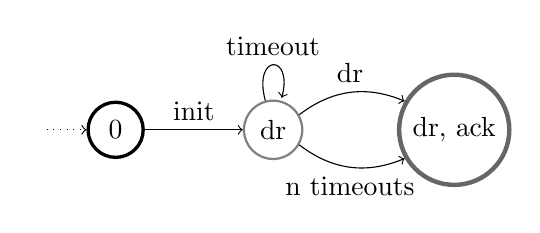
\begin{tikzpicture}
[
init/.style={circle, draw=black!100, very thick, minimum size=7mm,node distance=2cm},
state_split/.style={circle split, draw=gray!100, thick, minimum size=7mm,node distance=2cm},
state/.style={circle, draw=gray!100, thick, minimum size=7mm,node distance=2cm},
final/.style={circle, draw=black!60,  ultra thick, minimum size=10mm,node distance=23mm}
]
%Nodes
\node[init]         (start)                         {0};
\node               (em)        [left of=start]     {};
\node[state]        (send_dr)   [right of=start]    {dr};
\node[final]        (dc_ack)    [right of=send_dr]  {dr, ack};


%Lines
%\draw[->] (start.east) -- (synx.west);
%\draw[->] (synx.east) -- (end.west);
%\path[->] (start)  edge [loop above] node {a} (start); 
\draw[dotted, ->] (em.east) -- (start.west);
\path[->] 
(start)   edge                   node [above]   {init}      (send_dr)
(send_dr) edge [bend left]       node [above]   {dr}        (dc_ack)
(send_dr) edge [bend right]      node [below]   {n timeouts}  (dc_ack)
(send_dr) edge [loop above]      node           {timeout}   (send_dr);
\end{tikzpicture}

\\
Either the server or client should be able to initialize the teardown protocol.
\\
It do so by sending a disconnection request (dr) to the target host and at the same time start a timer. If it receives an ACK that the other host is disconnecting or after n timeout it will proceed to disconnect and send an ACK on this. 
\subsection{Teardown - Target host}
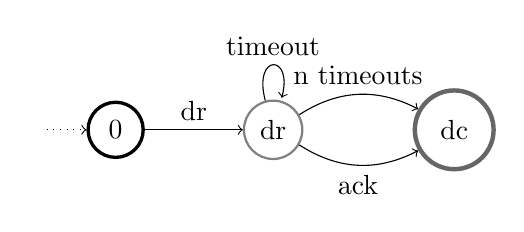
\begin{tikzpicture}
[
init/.style={circle, draw=black!100, very thick, minimum size=7mm,node distance=2cm},
state_split/.style={circle split, draw=gray!100, thick, minimum size=7mm,node distance=2cm},
state/.style={circle, draw=gray!100, thick, minimum size=7mm,node distance=2cm},
final/.style={circle, draw=black!60,  ultra thick, minimum size=10mm,node distance=23mm}
]
%Nodes
\node[init]         (start)                         {0};
\node               (em)        [left of=start]     {};
\node[state]        (send_dr)   [right of=start]    {dr};
\node[final]        (dc_ack)    [right of=send_dr]  {dc};


%Lines
%\draw[->] (start.east) -- (synx.west);
%\draw[->] (synx.east) -- (end.west);
%\path[->] (start)  edge [loop above] node {a} (start); 
\draw[dotted, ->] (em.east) -- (start.west);
\path[->] 
(start)   edge                   node [above]   {dr}    (send_dr)
(send_dr) edge [bend left]       node [above]   {n timeouts} (dc_ack)
(send_dr) edge [bend right]      node [below]   {ack}     (dc_ack)
(send_dr) edge [loop above]      node           {timeout}   (send_dr);
\end{tikzpicture}
\\
Here we have a problem, if all the disconnection requests sent from the initializing host get lost, the host will never know that it should disconnect, and that is something we just have to accept.
\\
However when the host receives the dr it will send a dr back and wait for an ACK, when it receives an ACK back or after n timeouts it will proceed to disconnect. 
\subsection{Sliding window sender state machine}
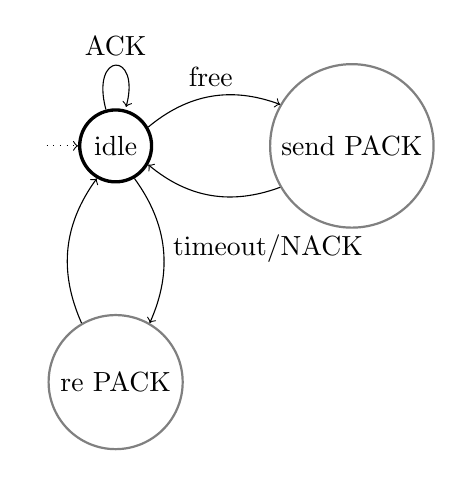
\begin{tikzpicture}
[
init/.style={circle, draw=black!100, very thick, minimum size=7mm,node distance=1cm},
state_split/.style={circle split, draw=gray!100, thick, minimum size=7mm,node distance=3cm},
state/.style={circle, draw=gray!100, thick, minimum size=7mm,node distance=3cm},
final/.style={circle, draw=black!60,  ultra thick, minimum size=10mm,node distance=23mm}
]
%Nodes
\node[init]     (start)                         {idle};
\node           (init)          [left of=start]     {};
\node[state]    (sack)          [right of=start]    {send PACK};
\node[state]    (reack)         [below of=start]    {re PACK};



%Lines
%\draw[->] (start.east) -- (synx.west);
%\draw[->] (synx.east) -- (end.west);
%\path[->] (start)  edge [loop above] node {a} (start); 
\draw[dotted, ->] (init.east) -- (start.west);
\path[->] 
          
(start) edge[bend left]         node[above]             {free}      (sack)
(sack)  edge[bend left]         node[below]             {}          (start)
(start) edge[bend left]         node[right]             {timeout/NACK} (reack)
(reack) edge[bend left]         node[left]              {}          (start)
(start) edge[loop above]        node[above]             {ACK}       (start);

\end{tikzpicture}
For the sliding windows itself it starts of in the idle state. If there is free space at the receiver end packages will be sent. If and when the ACK comes back nothing really happens. Sending more packages is based on having space on the receiver end and the ACK have information about how much space there is on the receiver end. If no ACK (selective) arrives on a sent package the package will be resent. There could be the possibility to receive a NACK to resend a specific. If a package is lost the receiver will still ACK packages after the lost one so only the lost package will be relly affected. 
\subsection{Sliding windew resiver satate machine}
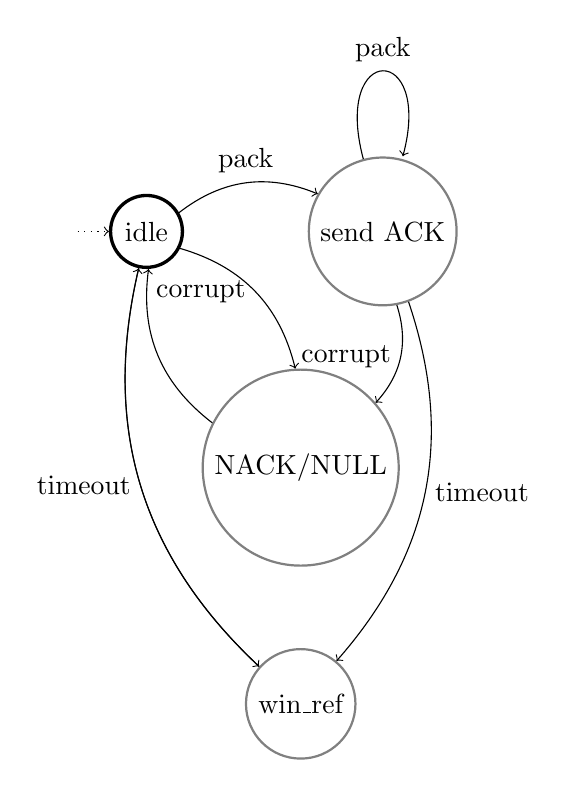
\begin{tikzpicture}
[
init/.style={circle, draw=black!100, very thick, minimum size=7mm,node distance=1cm},
state_split/.style={circle split, draw=gray!100, thick, minimum size=7mm,node distance=3cm,inner sep=0},
state/.style={circle, draw=gray!100, thick, minimum size=7mm,node distance=3cm},
final/.style={circle, draw=black!60,  ultra thick, minimum size=10mm,node distance=23mm}
]
%Nodes
\node[init]     (start)                         {idle};
\node           (init)          [left of=start]     {};
\node[state]    (ack)          [right of=start]    {send ACK};
\node[state]    (nack)         [below of=start, right=7mm]    {NACK/NULL};
%\node[state]    (wref)         [below of=nack]    {win_ref};
\node[state]    (wref)          [below of=nack]      {win\_ref};

%Lines
%\draw[->] (start.east) -- (synx.west);
%\draw[->] (synx.east) -- (end.west);
%\path[->] (start)  edge [loop above] node {a} (start); 
\draw[dotted, ->] (init.east) -- (start.west);
\path[->] 

(start) edge[bend left]                   node[above]             {pack}      (ack)
(start) edge [bend right]        node[left]             {timeout}   (wref)
(ack)   edge[loop above]        node[above]             {pack}      (ack)
(ack)   edge [bend left]        node[left]              {corrupt}   (nack)
(start) edge [bend left]        node[left]              {corrupt}   (nack)
(nack)  edge [bend left]        node                    {}          (start)
(ack)   edge [bend left]        node[right]             {timeout}   (wref)
(wref)  edge [bend left]        node                    {}          (start);





\end{tikzpicture}


\end{document}